\section{Kevin Natanel Nainggolan(117459)}
\subsection{Point Polyline dan Polygon}
\begin{enumerate}
	\item
	\lstinputlisting{src/1/1174059/pyshp1.py}
	\begin{figure}[H]
		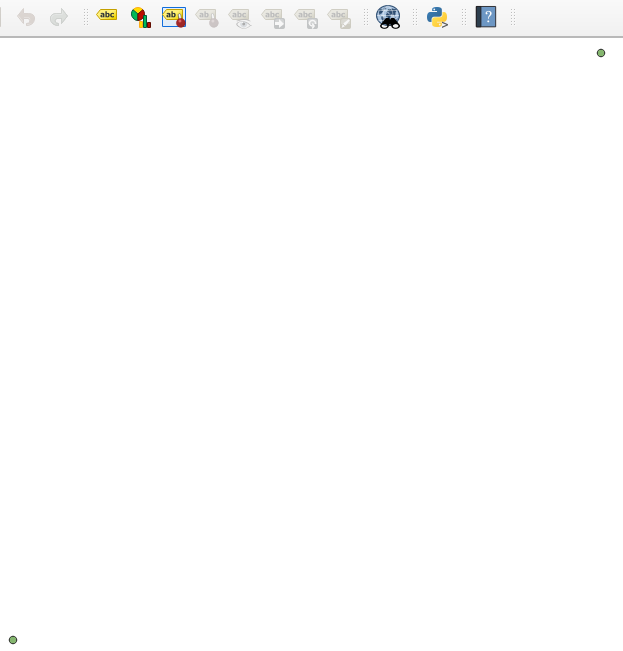
\includegraphics[width=12cm]{figures/1174059/Python1/soal1.PNG}
		\centering
		\caption{Point}
	\end{figure}
	
	\item 
	\lstinputlisting{src/1/1174059/pyshp2.py}
	\begin{figure}[H]
		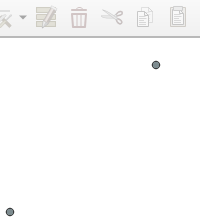
\includegraphics[width=12cm]{figures/1174059/Python1/soal2.PNG}
		\centering
		\caption{Point}
	\end{figure}
	
	\item 
	\lstinputlisting{src/1/1174059/pyshp3.py}
	\begin{figure}[H]
		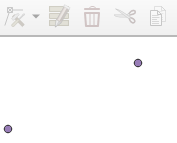
\includegraphics[width=12cm]{figures/1174059/Python1/soal3.PNG}
		\centering
		\caption{Point}
	\end{figure}
	
	\item 
	\lstinputlisting{src/1/1174059/pyshp4.py}
	\begin{figure}[H]
		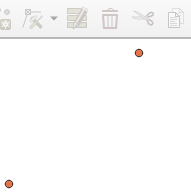
\includegraphics[width=12cm]{figures/1174059/Python1/soal4.PNG}
		\centering
		\caption{Point}
	\end{figure}
	
	\item 
	\lstinputlisting{src/1/1174059/pyshp5.py}
	\begin{figure}[H]
		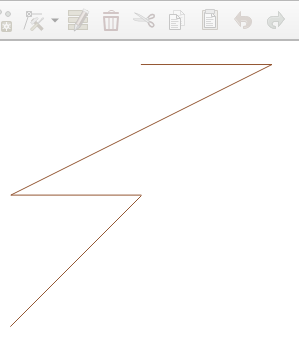
\includegraphics[width=12cm]{figures/1174059/Python1/soal5.PNG}
		\centering
		\caption{Polyline}
	\end{figure}
	
	\item 
	\lstinputlisting{src/1/1174059/pyshp6.py}
	\begin{figure}[H]
		
\includegraphics[width=12cm]{figures/1174059/Python1/soal6.PNG}
		\centering
		\caption{Poligon}
	\end{figure}
	
	\item 
	\lstinputlisting{src/1/1174059/pyshp7.py}
	\begin{figure}[H]
		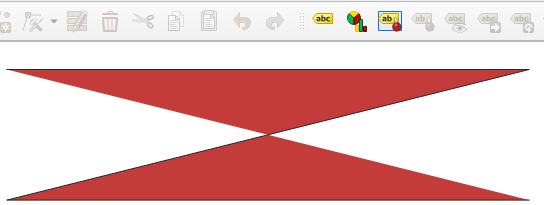
\includegraphics[width=12cm]{figures/1174059/Python1/soal7.PNG}
		\centering
		\caption{Polygon}
	\end{figure}
	
	\item 
	\lstinputlisting{src/1/1174059/pyshp8.py}
	\begin{figure}[H]
		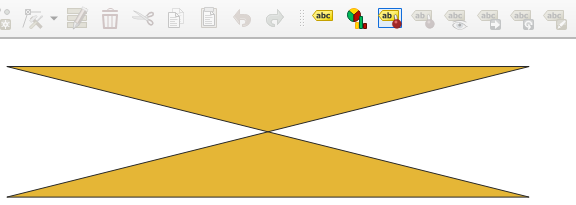
\includegraphics[width=12cm]{figures/1174059/Python1/soal8.PNG}
		\centering
		\caption{Polygon}
	\end{figure}
	
	\item 
	\lstinputlisting{src/1/1174059/pyshp9.py}
	\begin{figure}[H]
		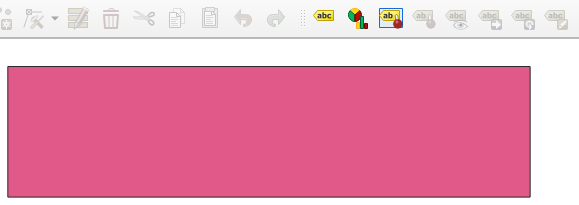
\includegraphics[width=12cm]{figures/1174059/Python1/soal9.PNG}
		\centering
		\caption{Polygon}
	\end{figure}

    \item 
	\lstinputlisting{src/1/1174059/pyshp10.py}
	\begin{figure}[H]
		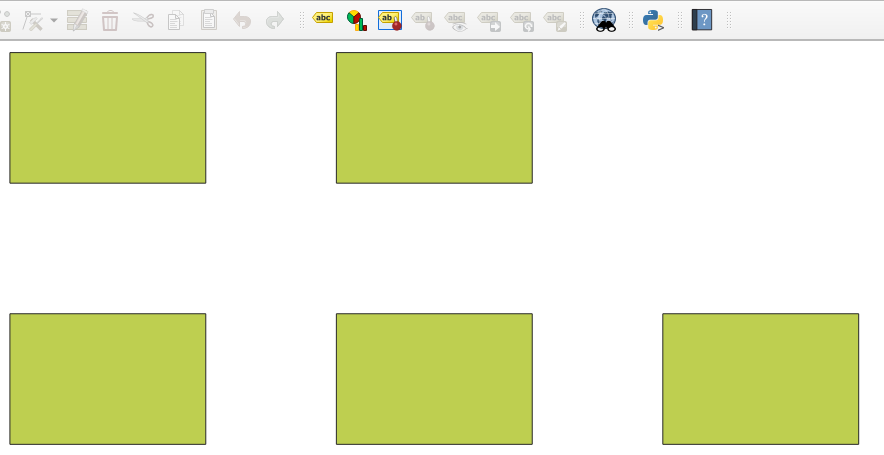
\includegraphics[width=12cm]{figures/1174059/Python1/soal10.PNG}
		\centering
		\caption{Hasil Mod saya 3 berberntuk persegi panjang sama kaki}
	\end{figure}
\end{enumerate}